\documentclass[a4paper,12pt]{article}
%%\documentclass[a4paper,
%%		     12pt,
%%		     DIV10,
%%		     DIVcalc,
%%		     headings=normal,
%%		     oneside,
%%		     bibliography=totoc,
%%		     headsepline=false,
%%		     headinclude]{scrartcl}

% font
\usepackage[utf8]{inputenc}
\usepackage[T1]{fontenc}
%\usepackage[automark,komastyle]{scrpage2}

% german; comment out if not needed
%\usepackage[ngerman]{babel}
%\usepackage[german]{varioref} 
%\usepackage{bibgerm}

% enlarge page size
\usepackage[a4paper,total={150mm,240mm}]{geometry}
%\usepackage[cm]{fullpage}

% often used packages
\usepackage{amsmath}
\usepackage{amsfonts}
\usepackage{amsthm}
\usepackage{amscd}
\usepackage{grffile}
\usepackage{tikz} 
\usepackage{eurosym} 
\usepackage{graphicx}
\usepackage{psfrag}
\usepackage{listings}
\lstset{language=C++, basicstyle=\ttfamily, 
  keywordstyle=\color{black}\bfseries, tabsize=4, stringstyle=\ttfamily,
  commentstyle=\it, extendedchars=true, escapeinside={/*@}{@*/}}
\usepackage{curves}
\usepackage{calc}
\usepackage{picinpar}
\usepackage{enumerate}
\usepackage{algorithmic}
\usepackage{algorithm}
\usepackage{bm}
\usepackage{multibib}
\usepackage{hyperref}
\usepackage{textcase}
\usepackage{nicefrac}

\theoremstyle{definition}
\newtheorem{Def}{Definition}
\newtheorem{Thm}[Def]{Theorem}
\newtheorem{Prop}[Def]{Proposition}
\newtheorem{Lem}[Def]{Lemma}
\newtheorem{Assumption}[Def]{Assumption}
\newtheorem{Exm}[Def]{Example}
\newtheorem{Obs}[Def]{Observation}
\newtheorem{Pro}[Def]{Proposition}
\newtheorem{Cor}[Def]{Corollary}
\newtheorem{Rem}[Def]{Remark}
\newtheorem{Alg}[Def]{Algorithm}
\newtheorem{Rep}[Def]{Repetition}

\definecolor{listingbg}{gray}{0.95}

\title{Tutorial 8\\ Unsteady Incompressible Navier-Stokes Equations}
\author{\textsc{Peter Bastian}\\
  Universität Heidelberg\\
  Interdisziplinäres Zentrum für Wissenschaftliches Rechnen\\
  Im Neuenheimer Feld 368, D-69120 Heidelberg\\
mail: \url{Peter.Bastian@iwr.uni-heidelberg.de}
}
\date{\today}

\begin{document}

\maketitle

\begin{abstract}
This tutorial provides a vanilla implementation of an unsteady incompressible Navier-Stokes
solver based on i) conforming Taylor-Hood finite elements, ii) grad-div stabilization to
improve satisfaction of the divergence constraint, iii) directional do-nothing condition
for improvement of the outflow boundary conditions and iv) Navier-slip condition for
modelling rough domains. In addition the transport of a dissolved
substance is computed which possibly interacts with the flow.
\end{abstract}

\tableofcontents

\newpage

\section{Incompressible Navier-Stokes Equations}

\subsection{Strong Form of the Equations}

We consider the incompressible Navier-Stokes equations in a $d$-dimensional domain $\Omega$ and time
interval $\Sigma$ which read in strong form \cite{JohnLectureNotes}:
\begin{subequations}
\begin{align}
\partial_t u + \nabla\cdot(u u^T)  &= \nabla \cdot \mathbb{S} + f &&\text{in $\Omega\times\Sigma$},\\
\mathbb{S} &= \nu \left( \nabla u + (\nabla u)^T \right) - pI,\\
\nabla\cdot u &= 0 .
\end{align}
\end{subequations}
Here $u:\Omega\times\Sigma\to\mathbb{R}^d$ is the unknown velocity field, 
$p:\Omega\times\Sigma\to\mathbb{R}$ is the unknown pressure (rescaled by constant mass density),
$\mathbb{S} = 2\nu\mathbb{D}(u)-pI$ is the stress tensor, $\nu$ is the kinematic viscosity,
$\mathbb{D}(u)=\frac12 \left( \nabla u + (\nabla u)^T \right)$ is the
symmetric velocity gradient and $f$ are external sources and sinks.

This model is equipped with the following boundary conditions:
\begin{subequations}
\begin{align}
u &= g                             &&\text{on $\Gamma_D$}, &&\text{(Dirichlet)}\\
\mathbb{S} n &= \frac12 (u\cdot n)_- u  &&\text{on $\Gamma_O$}, &&\text{(directional do-nothing)}\\
u\cdot n &= 0, \ n\times [\mathbb{S} n] \times n + \beta u = 0 &&\text{on $\Gamma_S$}. &&\text{(Navier slip)}
\end{align}
\end{subequations}
As usual, $n$ denotes the unit outer normal vector to the domain $\Omega$. The directional do-nothing condition, with 
$$(u\cdot n)_- = \left\{\begin{array}{ll}
0 & u\cdot n \geq 0,\\
(u\cdot n) & u\cdot n < 0,
\end{array} \right. $$ was introduced in \cite{Braack2014} with $\mathbb{S}$ replaced
by $\mathbb{T} = \nu \nabla u - pI$ and the form presented here is mentioned in \cite{JohnLectureNotes}.
The Navier slip condition is discussed in \cite{Neustupa2007}.

\begin{Rem}
This formulation is based in the symmetric gradient in order to be able to incorporate the
Navier slip condition. Moreover, in most formulations of the incompressible Navier-Stokes equations one exploits
the divergence constraint in the momentum equation leading to $2\nabla\cdot\mathbb{D}(u) = \nabla\cdot\nabla u + \nabla\cdot(\nabla u)^T
=  \nabla\cdot\nabla u + \nabla(\nabla\cdot u) =  \nabla\cdot\nabla u$ as well as $\nabla\cdot(uu^T) = (\nabla u) u + u (\nabla\cdot u)$. Since 
$\nabla\cdot u = 0$ does not hold in general in the discrete case we prefer to start from the formulation given here.
\end{Rem}

\subsection{Weak Formulation}

We recall the following compact notation for the $L_2$ inner product $$(f,g)_{0,\Omega} = \left\{\begin{array}{ll}
\int_\Omega fg \ dx & \text{$f,g$ scalar valued}\\
\int_\Omega f\cdot g \ dx & \text{$f,g$ vector valued}\\
\int_\Omega f : g \ dx & \text{$f,g$ matrix valued}
\end{array}\right. ,$$
and the integration by parts formula 
$$(\nabla\cdot\mathbb{A},v)_{0,\Omega} = - (\mathbb{A},\nabla v)_{0,\Omega} + (\mathbb{A}n,v)_{0,\partial\Omega}$$
for any matrix valued function $\mathbb{A}(x)$ and vector valued function $v(x)$.  

Then, for any test function with $v=0$ on $\Gamma_D$ we obtain the weak form of the momentum equation
\begin{equation*}
\begin{split}
(\partial_t u &+ \nabla\cdot(uu^T) - \nabla\cdot\mathbb{S},v)_{0,\Omega} = 
\partial_t( u,v )_{0,\Omega} + (\nabla\cdot(uu^T),v)_{0,\Omega} + (\mathbb{S},\nabla v)_{0,\Omega} - (\mathbb{S}n,v)_{0,\partial\Omega}\\
&= \partial_t( u,v )_{0,\Omega} + (\nabla\cdot(uu^T),v)_{0,\Omega} + 2\nu(\mathbb{D}(u),\nabla v)_{0,\Omega} - (p,\nabla\cdot v)_{0,\Omega}\\
& \qquad - \frac12 ( (u\cdot n)_- u , v)_{0,\Gamma_O} + \beta (u,v)_{0,\Gamma_S} \\
&= (f,v)_{0,\Omega} 
\end{split}
\end{equation*}
under the additional constraint $u\cdot n=0$ on $\Gamma_S$.
The weak form of the continuity equation reads for any test function $q$:
\begin{equation*}
(\nabla\cdot u , q)_{0,\Omega} = 0 .
\end{equation*}
Introducing the forms
\begin{align}
a(u,v) &= 2\nu(\mathbb{D}(u),\nabla v)_{0,\Omega} \\
b(u,q) &= -(\nabla\cdot u , q)_{0,\Omega},\\
c(u,w,v) &=  (\nabla\cdot(uw^T),v)_{0,\Omega} = ( (\nabla u)w , v )_{0,\Omega} + (u\cdot v, \nabla\cdot w)_{0,\Omega},\\
s(u,v) &=  \beta (u,v)_{0,\Gamma_S} - \frac12 ( (u\cdot n)_- u , v)_{0,\Gamma_O} 
\end{align}
and the function spaces
\begin{align}
V &= \left\{ v\in (H^1(\Omega))^d : \text{$v=0$ on $\Gamma_D$ and $v\cdot n=0$ on $\Gamma_S$} \right\},\\
U &= \left\{ u\in (H^1(\Omega))^d : \text{$u=u_g+v$, $v\in V$, $u_g=g$ on $\Gamma_D$, $u_g\cdot n=0$ on $\Gamma_S$} \right\},\\
Q &= \left\{ q\in L_2(\Omega) : \text{ $(q,1)_{0,\Omega}=0$ if $\Gamma_D=\partial\Omega$} \right\},
\end{align}
we obtain the following weak formulation. Find $(u,p)\in U\times Q$ such that
\begin{align}
\partial_t (u,v)_{0,\Omega} + c(u,u,v) + a(u,v) + b(v,p) + s(u,v)  &= (f,v)_{0,\Omega} &&\forall v\in V,\\
b(u,q) &= 0 &&\forall q\in Q.
\end{align}
\begin{Rem}
This weak formulation has the following properties:
\begin{itemize}
\item The boundary terms give a positive contribution when inserting $v=u$, i.e. $s(u,u) > 0$ for $u\neq 0$.
\item $a$ is a symmetric bilinear form since $(\nabla u)^T : \nabla v = \nabla u : (\nabla v)^T$.
\end{itemize}
\end{Rem}

\section{Finite Element Formulation}

We employ a conforming finite element method here, the so-called Taylor-Hood element. It uses the function spaces
\begin{align}
V_h &= \left\{ v\in (\mathbb{P}_{r+1})^d : \text{$v=0$ on $\Gamma_D$ and $v\cdot n=0$ on $\Gamma_S$} \right\},\\
U_h &= \left\{ u\in (\mathbb{P}_{r+1})^d : \text{$u=u_g+v$, $v\in V_h$, $u_g=g$ on $\Gamma_D$, $u_g\cdot n=0$ on $\Gamma_S$} \right\},\\
Q_h &= \left\{ q\in \mathbb{P}_r : \text{ $(q,1)_{0,\Omega}=0$ if $\Gamma_D=\partial\Omega$} \right\},
\end{align}
and is based on the following discrete weak formulation. Find $(u_h,p_h)\in U_h\times Q_h$ such that
{\small\begin{align}
\partial_t (u_h,v)_{0,\Omega} + c(u_h,u_h,v) + a(u_h,v) + b(v,p_h) + s(u_h,v) + \gamma (\nabla\cdot u_h, \nabla\cdot v) &= (f,v)_{0,\Omega}, \\
b(u_h,q) &= 0
\end{align}}
for all test functions $(v,q) \in V_h\times Q_h$.
 
\begin{Rem}
\begin{itemize}
\item Here, the grad-div stabilization was added with a factor $\gamma\geq 0$ in order to improve the pressure
robustness of the method, see the review \cite{John_etal_2017} on this topic.
\item The slip boundary condition is most simple to implement when $n$ points in the direction of a single coordinate.
\end{itemize}
\end{Rem}
Insertion of a basis representation results in a nonlinear algebraic
system which is solved with Newton's method and the linearized sub
problem is solved with a BiCG-Stab method preconditioned with
incomplete factorization.

\subsection{Preparations}

In order to speed up the computations for the finite element method we
aim at employing matrix-matrix computations as much as possible. The
general strategy is
\begin{itemize}
  \item Extract coefficients involved with one element from the global
    data structure.
  \item All element-wise sizes of arrays are known at compile-time.
  \item Compute quantities at quadrature points.
  \item Compute residual constributions.
\end{itemize}
We now collect some basic tools and introduce notation for
element-wise computations. Then the individual terms of the weak
formulation are treated.

\subsubsection*{Element Transformation}

Given an element $T\in\mathcal{T}_h$ the transformation from the reference element to the real element is denoted by $T = \mu_T(\hat T)$
with the Jacobian inverse transposed $J_T(\hat x) = \nabla\mu_T^{-T}(\hat x)$.

\subsubsection*{Basis Functions and Gradients} 

For polynomial degree $r$ introduce the global basis functions
\begin{equation}
\mathbb{P}_{r+1}=\text{span}\{ \phi_1,\ldots,\phi_{N_u}\}, \qquad 
\mathbb{P}_{r}=\text{span}\{ \psi_1,\ldots,\phi_{N_p}\}
\end{equation}
and then set
\begin{equation}
(\mathbb{P}_{r+1})^d = \text{span}\left\{ \Phi_{i,k} = \phi_k e_i, 1\leq k \leq N_u, 1\leq i \leq d    \right\}
\end{equation}
with the unit vectors $(e_i)_j=\delta_{ij}$. Using that notation we have
\begin{equation}
u_h(x) = \sum_{l=1}^{N_u} \sum_{j=1}^d z_{j,l} \phi_l e_j, \qquad p_h(x) = \sum_{m=1}^{N_p} y_{m}\psi_m(x)
\end{equation}

The basis function $\phi_k$ at a point $T\ni x = \mu_{T}(\hat x)$
is generated from a basis function $\hat\phi_l$ on the reference element via $\phi_k(\mu_T(\hat x)) = \hat\phi_l(\hat x)$ 
and we define the vector of local basis function evaluations
$$ \hat \phi(\hat x) = \left( \hat\phi_1(\hat x),\ldots,\hat\phi_{n_u}(\hat x) \right)^T, \qquad
\hat\psi(\hat x) =  \left( \hat\psi_1(\hat x),\ldots,\hat\psi_{n_p}(\hat x) \right)^T$$
where $n_u=n_{r+1}$ is the number of basis functions of velocity space on the reference element and
$n_p=n_r$ is the number of pressure basis functions on the reference element.
Then we can evaluate
\begin{equation}
\label{eq:evalu}
\begin{split}
u_h(x) &=  \sum_{l=1}^{n_u} \sum_{j=1}^d z_{j,l}   \phi_l(x) e_j  = \sum_{l=1}^{n_u} \phi_l(x) \left(\begin{array}{c}
z_{1,l}\\ \vdots\\ z_{d,l} \end{array}\right)
= Z_T \hat\phi(\hat x)
\end{split}
\end{equation}
where $(Z_T)_{j,l} = z_{j,l}$ is the matrix of coefficients on element $T$.
In a similar way the pressure on an element is evaluated as
\begin{equation}
\label{eq:evalp}
\begin{split}
p_h(x) &=  \sum_{m=1}^{n_p} y_{m} \psi_m(x) 
= Y_T \cdot \hat\psi(\hat x)
\end{split}
\end{equation}
where $Y_T$ is the vector of pressure degrees of freedom on element $T$.

For the gradients we define the matrices (no gradients of pressure basis functions is needed)
$$\hat G(\hat x) = \left[ \hat\nabla\hat\phi_1,\ldots,\hat\nabla\hat\phi_{n_u}\right] \qquad \text{and} \qquad
G_T(x) = J_T(\hat x) \hat G(\hat x)$$
and now seek to compute $\nabla u(x) $ for $T\ni x = \mu_{T}(\hat x)$:
\begin{equation}
\label{eq:evalgradu}
\begin{split}
\nabla u_h(x) &=  \sum_{l=1}^{n_u} \sum_{j=1}^d z_{j,l} \nabla(  \phi_l(x) e_j ) 
= \sum_{l=1}^{n_u} \sum_{j=1}^d z_{j,l} e_j (\nabla\phi_l(x))^T\\
&= \sum_{l=1}^{n_u} \left(\sum_{j=1}^d  z_{j,l} e_j\right)  (J_T(\hat x) \hat\nabla\hat\phi_l(\hat x) )^T
= \sum_{l=1}^{n_u} z_{\ast,l}  (J_T(\hat x) \hat\nabla\hat\phi_l(\hat x) )^T\\
&= Z_T G^T_T(x) = Z_T  ({\hat G}(\hat x))^T J^T_T(\hat x) .
\end{split}
\end{equation}
 
Now for the divergence:
\begin{equation}
\label{eq:evaldivu}
\begin{split}
\nabla\cdot u_h(x) &=  \sum_{l=1}^{n_u} \sum_{j=1}^d z_{j,l} \nabla\cdot(  \phi_l(x) e_j ) 
= \sum_{l=1}^{n_u} \sum_{j=1}^d z_{j,l} \partial_{x_j} \phi_l(x) 
= \sum_{l=1}^{n_u} \sum_{j=1}^d z_{j,l} (G_T(x))_{j,l} = Z_T : G_T(x).
\end{split}
\end{equation}
 

\subsubsection*{Quadrature}

The integral of a function $q : T \to\mathbb{R}$ is approximated by a generic quadrature rule
\begin{equation}
\int_T q(x)\,dx = \int_{\hat T} q(\mu_T(\hat x))  \text{det} \nabla\mu_T(\hat x) \,d\hat x
= \sum_{\alpha=1}^{M_T} q(\mu_T(\hat x_\alpha))  \text{det} \nabla\mu_T(\hat x_\alpha)  \hat w_\alpha + \text{error}.
\end{equation}
The weights are collected in the column vector $w_T\in\mathbb{R}^M$ with $(w_T)_\alpha = 
\text{det} \nabla\mu_T(\hat x_\alpha)  \hat w_\alpha$.

Boundary integrals are treated in a similar way. Let $F$ be a face of element $T\in\mathcal{T}_h$. $F$ has the reference
element $\hat F$ and there are two maps $\eta_F : \hat F \to F$ and $\xi_{F,T} : \hat F \to \hat T$ that satisfy
$\eta_F(\hat s) = \mu_T( \xi_{F,T}(\hat s) )$. Then the integral of a function $q : T \to\mathbb{R}$ over the
face $F$ of $T$ can be computed by
\begin{equation}
\int_F q(s) \,ds = \int_{\hat F} q(\mu_T(\xi_{F,T}(\hat s))) \Delta_{F,T}(\hat s) \, d\hat s
= \sum_{\alpha=1}^{M_F} q(\mu_T(\xi_{F,T}(\hat s_\alpha))) \Delta_{F,T}(\hat s_\alpha) \hat w_\alpha + \text{error}
\end{equation}
with the integration element $\Delta_{F,T}(\hat s) = \sqrt{|\text{det}\left((\nabla\eta(\hat s))^T \nabla\eta(\hat s)\right)|}$.
We collect the weights in the vector $(w_F)_\alpha = \Delta_{F,T}(\hat s_\alpha) \hat w_\alpha$.

\subsection{Element Integrals}

\subsubsection*{Stress Term}

For element $T\in\mathcal{T}_h$ we seek to compute the integrals 
$$(R^\mathbb{S}_T)_{i,k} = 2\nu(\mathbb{D}(u),\nabla\Phi_{i,k})_{0,T}$$ for all test functions $\Phi_{i,k}$
with support intersecting $T$. $R^\mathbb{S}_T$ is represented as a $d\times n_u$ matrix.

Using the representation of $\nabla u(x)$ from \eqref{eq:evalgradu} we obtain
\begin{equation}
S_T(x) = 2\mathbb{D}(u)(x) = \nabla u(x) + (\nabla u(x))^T
= Z_T G^T_T(x) + G_T(x) Z^T_T 
\end{equation}
and may compute
\begin{equation*}
\begin{split}
\left(R^\mathbb{S}_T \right)_{i,k} &= 2\nu \int_T \mathbb{D}(u) : \nabla\Phi_{i,k} \, dx
= \nu \int_T (\nabla u + (\nabla u)^T) :( e_i (\nabla\phi_k)^T) \, dx \\
&= \nu \int_T \nabla u_i \cdot \nabla\phi_k + \partial_i u \cdot \nabla\phi_k \, dx
\end{split}
\end{equation*}
which gives for a column
\begin{equation*}
\begin{split}
\left(R^\mathbb{S}_T \right)_{\ast,k} 
&= \nu \int_T \nabla u \cdot \nabla\phi_k + (\nabla u)^T \nabla\phi_k \, dx
= 2\nu \int_T \mathbb{D}(u) \nabla\phi_k \, dx,
\end{split}
\end{equation*}
and results in
\begin{equation}
\begin{split}
R^\mathbb{S}_T &= 2\nu \int_T \mathbb{D}(u) G_T(x) \, dx = \nu \int_T S_T(x) G_T(x) \, dx 
\approx \nu \sum_\alpha S_T(x_\alpha) G_T(x_\alpha) (w_T)_\alpha
\end{split}
\end{equation}
after inserting quadrature.

\subsubsection*{Grad-Div Stabilization Term}

For element $T\in\mathcal{T}_h$ we seek to compute the integrals 
$(R^{\nabla\nabla\cdot}_T)_{i,k} = (\nabla\cdot u,\nabla\cdot\Phi_{i,k})_{0,T}$ for all test functions $\Phi_{i,k}$
with support intersecting $T$. $R^C_T$ is represented as a $d\times n_u$ matrix. Observe
\begin{equation*}
(R^{\nabla\nabla\cdot}_T)_{i,k} = \left(\nabla\cdot u,\Phi_{i,k}\right)_{0,T} 
= \left(\nabla\cdot u,\nabla\cdot(\phi_{k}e_i) \right )_{0,T} 
= \left(\nabla\cdot u, \partial_{x_i}\phi_{k} \right )_{0,T} 
= \left(\nabla\cdot u, (G_T)_{i,k} \right )_{0,T} 
\end{equation*}
and therefore
\begin{equation*}
\begin{split}
R^{\nabla\nabla\cdot}_T &= \int_T \nabla\cdot u(x) G_T(x)  \,dx
\approx \sum_\alpha (Z_T : G_T(\mu_T(\hat x_\alpha)) G_T(\mu_T(\hat x_\alpha)) (w_T)_\alpha
\end{split}
\end{equation*}

\subsubsection*{Pressure Term}

For element $T\in\mathcal{T}_h$ we seek to compute the integrals 
$(R^{p}_T)_{i,k} = ( p, \nabla\cdot\Phi_{i,k})_{0,T}$ for all test functions $\Phi_{i,k}$
with support intersecting $T$. $R^p_T$ is represented as a $d\times n_u$ matrix:
\begin{equation*}
(R^{p}_T)_{i,k} = \left( p,\nabla\cdot\Phi_{i,k}\right)_{0,T} =  \left( p,\partial_{x_i}\phi_{k}\right)_{0,T} 
=  \left( p, (G_T(x))_{i,k} \right)_{0,T}
\end{equation*}
which gives in matrix form:
\begin{equation}
R^{p}_T = \int_{\hat T} p(\mu_T(\hat x)) G_T(\mu_T(\hat x) ) \, \text{det} \nabla\mu_T(\hat x) \,d\hat x
\approx \sum_\alpha (Y_T \cdot \hat\psi(\hat x_\alpha) ) G_T(\mu_T(\hat x_\alpha))  (w_T)_\alpha
\end{equation}

\subsubsection*{Convection Term}

For element $T\in\mathcal{T}_h$ we seek to compute the integrals 
$(R^C_T)_{i,k} = (\nabla\cdot(uu^T),\Phi_{i,k})_{0,T}$ for all test functions $\Phi_{i,k}$
with support intersecting $T$. $R^C_T$ is represented as a $d\times n_u$ matrix.
Using the product rule $\nabla\cdot(uu^T)(x) = \nabla u(x) u(x) + u(x) \nabla\cdot u(x)$ we can reuse \eqref{eq:evalu},  \eqref{eq:evalgradu},
\eqref{eq:evaldivu}:
\begin{equation*}
(R^C_T)_{i,k} = \left(\nabla\cdot(uu^T),\Phi_{i,k}\right)_{0,T} = \left(\nabla\cdot(uu^T),\phi_{k}e_i \right )_{0,T} = 
\left(\left[\nabla\cdot(uu^T)\right]_i,\phi_{k}\right)_{0,T}
\end{equation*}
and therefore
\begin{equation}
\begin{split}
R^C_T &= \int_T \nabla\cdot(uu^T) \hat\phi^T(\hat x) \text{det} \nabla\mu_T(\hat x) \,dx\\
&\approx \sum_\alpha \left[  \nabla u_h(\mu_T(\hat x_\alpha)) \hat u_h(\hat x_\alpha) 
+ \hat u_h(\hat x_\alpha) \nabla\cdot u_h(\mu_T(\hat x_\alpha)) \right] \hat\phi^T(\hat x_\alpha) (w_T)_\alpha.
\end{split}
\end{equation}

\begin{Rem}
The efficient evaluation of this expression should follow the rules:
\begin{itemize}
\item Do a right to left evaluation to minimize flop count.
\item Vectorize over quadrature points.
\end{itemize}
\end{Rem}

\subsubsection*{Mass Term}

For element $T\in\mathcal{T}_h$ we seek to compute the integrals 
$(R^{M}_T)_{i,k} = ( u, \Phi_{i,k})_{0,T}$ for all test functions $\Phi_{i,k}$
with support intersecting $T$. $R^M_T$ is represented as a $d\times n_u$ matrix:
\begin{equation*}
(R^{M}_T)_{i,k} = \left( u,\Phi_{i,k}\right)_{0,T} =  \left( u,\phi_{k} e_i\right)_{0,T} =  \left( u\cdot e_i,\phi_{k}\right)_{0,T}
\end{equation*}
which gives in matrix form
\begin{equation}
R^{M}_T = \int_{\hat T} u(\mu_T(\hat x)) \hat\phi^T(\hat x)  \, \text{det} \nabla\mu_T(\hat x) \,d\hat x
\approx \sum_\alpha (Z_T \hat\phi(\hat x_\alpha)) \hat\phi^T(\hat x_\alpha) (w_T)_\alpha
\end{equation}


\subsubsection*{External Force Term}

For element $T\in\mathcal{T}_h$ we seek to compute the integrals 
$(R^{f}_T)_{i,k} = ( f, \Phi_{i,k})_{0,T}$ for all test functions $\Phi_{i,k}$
with support intersecting $T$. $R^f_T$ is represented as a $d\times n_u$ matrix:
\begin{equation*}
(R^{f}_T)_{i,k} = \left( f,\Phi_{i,k}\right)_{0,T} =  \left( f,\phi_{k} e_i\right)_{0,T} =  \left( f\cdot e_i,\phi_{k}\right)_{0,T}
\end{equation*}
which gives in matrix form
\begin{equation}
R^{f}_T = \int_{\hat T} f(\mu_T(\hat x)) \hat\phi^T(\hat x)  \, \text{det} \nabla\mu_T(\hat x) \,d\hat x
\approx \sum_\alpha f(\mu_T(\hat x_\alpha)) \hat\phi^T(\hat x_\alpha) (w_T)_\alpha
\end{equation}

\subsubsection*{Divergence Term}

For element $T\in\mathcal{T}_h$ we seek to compute the integrals 
$(R^{\nabla\cdot}_T)_{k} = ( \nabla\cdot u, \psi_{k})_{0,T}$ for all pressure test functions $\psi_{k}$
with support intersecting $T$. $R^{\nabla\cdot}_T$ is represented as a column vector with $n_p$ components:
\begin{equation*}
(R^{\nabla\cdot}_T)_{k} = \left( \nabla\cdot u,\psi_{k}\right)_{0,T} 
= \left( Z_T:G_T,\psi_{k}\right)_{0,T} 
\end{equation*}
which gives 
\begin{equation*}
R^{\nabla\cdot}_T = \int_{\hat T} (Z_T : G_T(\mu_T(\hat x))) \hat\psi(\hat x) \, \text{det} \nabla\mu_T(\hat x) \,d\hat x
\approx \sum_\alpha  (Z_T : G_T(\mu_T(\hat x_\alpha))) \hat\psi(\hat x_\alpha) (w_T)_\alpha
\end{equation*}

\subsubsection*{Navier Slip Boundary Term}

For boundary face $F$ of element $T\in\mathcal{T}_h$ we seek to compute the integrals 
$(R^{S}_T)_{i,k} = \beta ( u , \Phi_{i,k})_{0,F}$ for all test functions $\Phi_{i,k}$
with support intersecting $T$. $R^{S}_T$ is represented as a $d\times n_u$ matrix:
\begin{equation*}
(R^{S}_T)_{i,k} = \beta ( u , \Phi_{i,k})_{0,F} = \beta ( u , \phi_{k}e_i )_{0,F} = \beta ( u\cdot e_i , \phi_{k} )_{0,F} ,
\end{equation*}
so
\begin{equation}
R^{S}_T = \beta \int_{\hat F} u(\mu_T(\xi_{F,T}(\hat s)))  \hat\phi^T(\xi_{F,T}(\hat s)) \Delta_{F,T}(\hat s) \,d\hat s
\approx \sum_\alpha (Z_T \hat\phi(\xi_{F,T}(\hat s_\alpha))) \hat\phi^T(\xi_{F,T}(\hat s_\alpha))  (w_F)_\alpha .
\end{equation}


\subsubsection*{Directional Do-Nothing Boundary Term}

For boundary face $F$ of element $T\in\mathcal{T}_h$ we seek to compute the integrals 
$(R^{O}_T)_{i,k} = \frac12 ( (u\cdot n)_-u, \Phi_{i,k})_{0,F}$ for all test functions $\Phi_{i,k}$
with support intersecting $T$. $R^{O}_T$ is represented as a $d\times n_u$ matrix:
\begin{equation*}
(R^{O}_T)_{i,k} = \frac12 ( (u\cdot n)_-u  , \Phi_{i,k})_{0,F} = \frac12 ( (u\cdot n)_- (u\cdot e_i), \phi_{k} )_{0,F} ,
\end{equation*}
so
\begin{equation}
\begin{split}
R^{O}_T &= \frac12 \int_{\hat F} (u(\mu_T(\xi_{F,T}(\hat s)))\cdot n)_- u(\mu_T(\xi_{F,T}(\hat s)))  \hat\phi^T(\xi_{F,T}(\hat s)) \Delta_{F,T}(\hat s) \,d\hat s\\
&\approx \sum_\alpha ( (Z_T \hat\phi(\xi_{F,T}(\hat s_\alpha))) \cdot n)_- (Z_T \hat\phi(\xi_{F,T}(\hat s_\alpha))) \hat\phi^T(\xi_{F,T}(\hat s_\alpha))  (w_F)_\alpha .
\end{split}
\end{equation}

\section{Realization in PDELab}

The structure of the code is very similar to that of tutorial 00. It was the aim to implement all computations
as efficient as possible while still being flexible in the choice of the degree of the basis functions and
the quadrature points (this was not done in tutorial 00). 
There are actually four examples in tutorial 08 which are called
\begin{center}
\lstinline{navier-stokes-}\textit{example}
\end{center}
with
\begin{center}
\textit{example} $\in$ \{ \lstinline{driven-cavity}, \lstinline{driven-cavity-3d}, \lstinline{cylinder}, \lstinline{rayleigh-benard}\}.
\end{center}
All examples, except the second one, are two-dimensional.
There are the following files:
\begin{enumerate}[1)]
\item For every example there is a \lstinline{.cc} file setting up initial and boundary conditions for the
specific example and calling the driver.
\item For every example there is a corresponding \lstinline{.ini} file holding parameters read by various parts of the code.
\item File \lstinline{driver_flow.hh} has a function \lstinline{driver_flow} which instantiates the necessary PDELab classes 
for solving the nonlinear instationary problem and then solves the problem and outputs results.
\item File \lstinline{driver_coupled.hh} contains a function \lstinline{driver_coupled} that instantiates the necessary PDELab classes 
for solving the nonlinear instationary problem as well as the transport problem for a dissolved component.
The transport problem is coupled to the flow problem via the velocity field while the flow problem
may be coupled to the transport problem e.g. through a concentration-dependent density. The transport problem 
is discretized with a discontinuous Galerkin method implemented in \lstinline{dune-pdelab} and the coupled
problem is solved with first-order operator splitting.
\item File \lstinline{navier-stokes-lop} contains the class
\lstinline{ConformingNavierStokesLOP} realizing a PDELab local operator implementing
the conforming finite element method for a given order and element type.
So far, the jacobians are computed via numerical differentiation. Since the
run-time of the code is limited by the linear solvers there is not much to gain
with analytical jacobians without implementing a faster solver.
\item File \lstinline{schemes.hh} implements several classes that can be used to parametrize the driver for various orders
and element types. 
\item File \lstinline{timecapsule.hh} implements a simple helper class required for time-dependent boundary conditions.
\item Finally, the tutorial provides some mesh files.
\end{enumerate}

\subsection{Compilation Control}

All examples use the UG grid manager for their computations.
In order to cut down on compilation time the executable is compiled for exactly one configuration
of dimension, element / mesh type and polynomial degree. The configuration is controlled by three compile time constants:
\lstinputlisting[linerange={68-70}, basicstyle=\ttfamily\small,
frame=single,
backgroundcolor=\color{listingbg}]{../src/navier-stokes-driven-cavity.cc}
When the constant \lstinline{STRUCTURED} is defined, an equidistant structured mesh is used with
parameters set in the inifile (see below). When \lstinline{CUBE} is defined then quadrilateral or
hexahedral meshes are used, otherwise triangles or tetrahedra.
Note that the dimension is fixed by the example itself. Only the \lstinline{driven-cavity-3d}
example works in three dimensions, all other examples are two-dimensional. 
If \lstinline{STRUCTURED} is not defined a gmsh file is read which may contain a cuboid or
a simplicial mesh. In that case be sure to still set (or undef) \lstinline{CUBE} to chose the correct finite element space.
Finally, the constant \lstinline{DEGREE}
selects the polynomial degree used for velocity. Pressure is always one degree less and concentration uses
the same degree as velocity. Note that on cube meshes only degree 2 is valid and on simplicial meshes degrees 2 and 3
are supported. New schemes can be defined by the user, see the examples
in the file \lstinline{schemes.hh}. There the number of quadrature
points has to be chosen appropriately with respect to the polynomial
degree. See table \ref{table:quadrature} for a correspondance between
quadrature order and number of quadrature points.

\subsection{Ini-File}

The ini-file allows the user to set various run-time parameters for the
execution of the program. Here we skim briefly through the sections of the
parameters of the coupled flow problem givewn in the file \lstinline{navier-stokes-rayleigh-benard.ini}.
\lstinputlisting[basicstyle=\ttfamily\small,
frame=single,
backgroundcolor=\color{listingbg}]{../src/navier-stokes-rayleigh-benard.ini}
The  \lstinline{[grid]} section controls the grid that is used for the computations.
If the program is compiled for a structured mesh then the keys \lstinline{extend}
and \lstinline{cells} are relevant. These give the extend of the domain in $x$ and $y$ direction
as well as the number of cells in $x$ and $y$ direction. In the case of an unstructured mesh the
name of the meshfile is given by the key \lstinline{meshfile}. Then, \lstinline{refinement} gives
the number of uniform refinement steps and is applicable to both types of meshes.

The \lstinline{[problem]} section determines the parameters of the PDE and its discrete
weak formulation:

\begin{tabular}{rl}
\texttt{viscosity} &  dynamic viscosity $\nu$ in Navier-Stokes equations\\
\texttt{gamma} & $\gamma$ in grad-div stabilization\\
\texttt{beta} & $\beta$ in Navier slip condition (not used here)\\
\texttt{dt} & time step size\\
\texttt{T} & length of time interval\\
\texttt{heatconductivity} & diffusion parameter $\kappa$ in transport problem\\
\texttt{rho\_0} & density for concentration zero\\
\texttt{alpha} & expansion coefficient 
\end{tabular}

The force density in the Navier-Stokes equation is $f = - \varrho(c) e_z$ where $e_z=(0,1)^T$ points
vertically up and $\varrho(c) = \varrho_0 - \alpha c$ describes the linear dependence of density on
concentration (or rather temperature here). For this setup (with a domain of size 1) we have
\begin{equation*}
Pr = \frac{\nu}{\kappa}, \qquad Ra = \frac{\alpha}{\nu\kappa},
\end{equation*}
where $Pr$ is the Prandtl number and $Ra$ is the Rayleigh number.

The \lstinline{[solver]} section sets some parameters controlling the operation of the
nonlinear (Newton) and linear (ILU-preconditioned BiCGStab) solvers.

\begin{tabular}{rl}
\texttt{lineariterationsmax} &  max. BiCGStab iterations allowed\\
\texttt{linearsolververbosity} & amount of output of linear solver\\
\texttt{nonlinearabslimit} & smallest absolute residual norm in Newton\\
\texttt{nonlinearreduction} & relative reduction required in Newton\\
\texttt{linearreduction} & relative reduction required for BiCGStab
\end{tabular}

\begin{figure}
\begin{center}
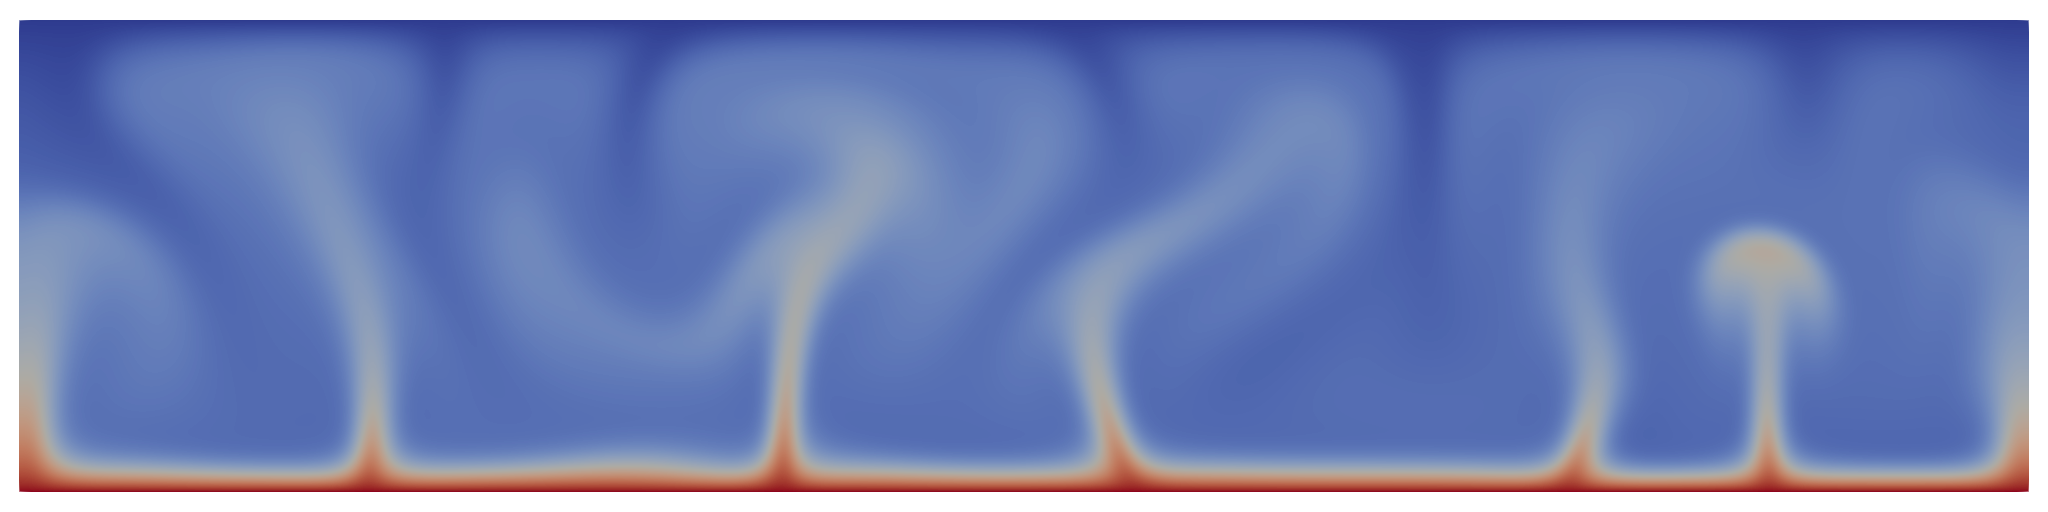
\includegraphics[width=\textwidth]{rayleighbenard1.png}\\
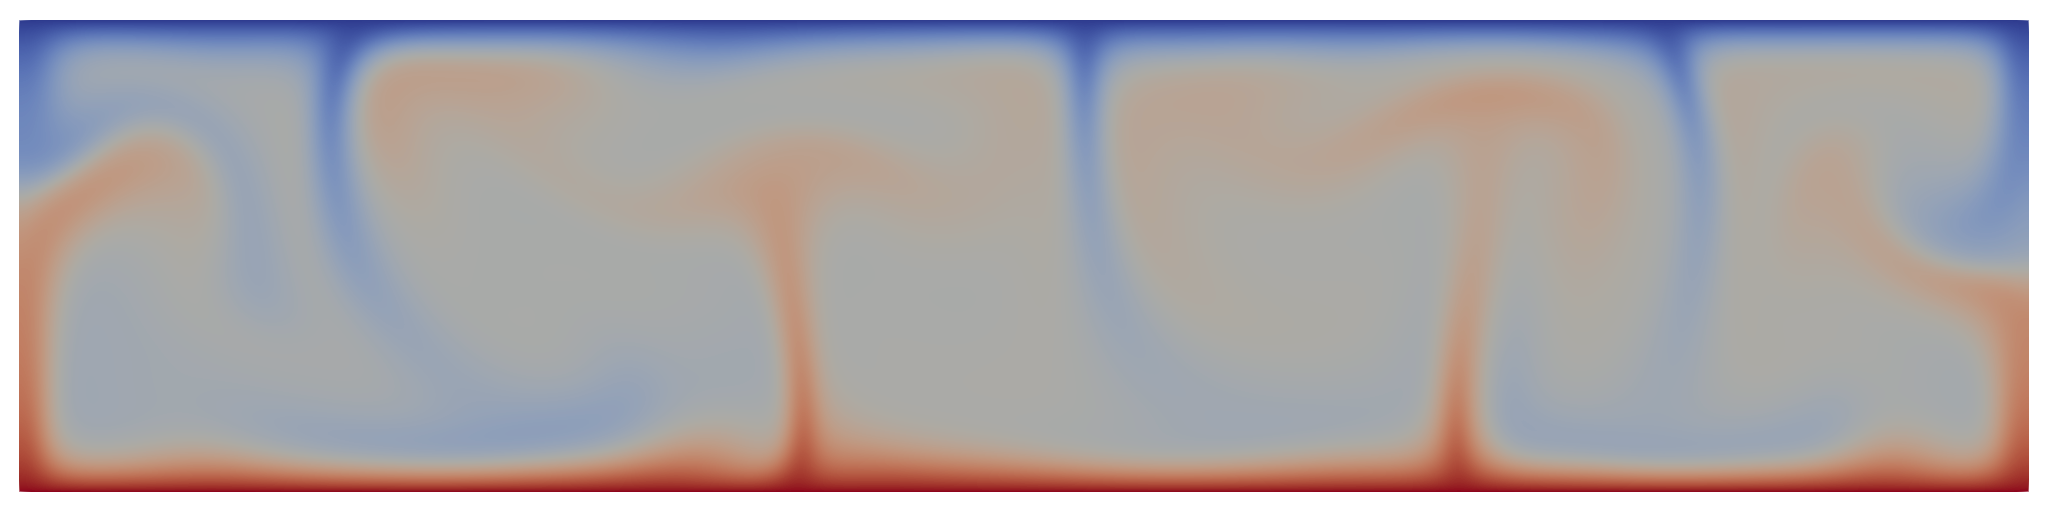
\includegraphics[width=\textwidth]{rayleighbenard2.png}
\end{center}
\caption{Rayleigh-Bénard flow for $Ra=4\cdot 10^7$ and $Pr=40$. Top image is from the early phase and the
bottom image is after establishment of convection rolls. The solution does not become stationary.}
\end{figure}

Finally, the \lstinline{[output]} section controls the VTK output of the simulation by setting the name of the
various output files, selecting the subsampling depth mesh refinement during output and restricting output to the 
timesteps numbers divisible by \lstinline{every}.

\begin{table}
\caption{Number of quadrature points for a given order (polynomial
  degree that is integrated exactly) depending on the element type. In
the implementation the number of quadrature points needs to be
provided at compile-time.}
\label{table:quadrature}
\begin{center}
\begin{tabular}{rrrrrr}
\hline
order & line & tri & quad & tet & hex \\
 \hline
    1  &  1 &   1  &   1   &   1    &   1        \\
    2  & 2  &   3  &   4    &  4    &   8        \\
    3 &  2 &    4  &   4    &  8    &   8        \\
    4 &  3 &    6  &   9    &  15   &   27       \\
    5  & 3  &   7  &   9    &  15   &   27       \\
    6 &  4 &    12  &  16  &   60  &  64     \\
    7  &  4 &   12 &   16   &  60  &  64     \\
    8  & 5  &   16 &   25    & 96  &  125    \\
    9  &  5 &   19  &  25   &   114 & 125    \\
    10  & 6  &   25 &   36  &  175 & 216   \\
    11  &  6 &   28 &   36  &  196 & 216   \\
    12 & 7  &    33 &   49  &  264 & 343   \\
    13 & 7  &    56 &   49  &  448 & 343   \\
    14  & 8  &   64 &   64  &  576 & 512   \\
    15  &  8 &   72 &   64  &  648 & 512   \\
    16 & 9  &    81 &   81  &  810 & 729   \\
    17 &  9 &    90 &   81  &  900 & 729   \\
    18  & 10  &   100 &  100 &  1100 & 1000\\
    19 &  10 &    110 &  100  & 1210 & 1000\\
  20   &  11 &  121  & 121   &  1452 & 1331\\
  \hline
\end{tabular}
\end{center}
\end{table}

% bibtex bibliography
\bibliographystyle{plain}
\bibliography{tutorial08.bib}

\end{document}
